%\addchap{Anhang A}
%\setcounter{chapter}{1}
%
%\section{Details zu bestimmten theoretischen Grundlagen}
%
%\section{Weitere Details, welche im Hauptteil den Lesefluss behindern}
%
%\addchap{Anhang B}
%\setcounter{chapter}{2}
%\setcounter{section}{0}
%\setcounter{table}{0}
%\setcounter{figure}{0}
%
%\section{Versuchsanordnung}
%
%\section{Liste der verwendeten Messgeräte}
%
%\section{Übersicht der Messergebnisse}
%
%\section{Schaltplan und Bild der Prototypenplatine}

%\clearpage
%
%Diese Seite wurde eingefügt, um zu zeigen, wie sich der Inhalt der Kopfzeile automatisch füllt.
%
%\addchap{Anhang C}
%\setcounter{chapter}{3}
%\setcounter{section}{0}
%\setcounter{table}{0}
%\setcounter{figure}{0}
%
%\section{Struktogramm des Programmentwurfs}
%
%\section{Wichtige Teile des Quellcodes}
%
\addchap{Anhang A}
\setcounter{chapter}{1}
\setcounter{section}{1}
\setcounter{table}{0}
\setcounter{figure}{0}
%
%\section{Einbinden von PDF-Seiten aus anderen Dokumenten}
%
%Auf den folgenden Seiten wird eine Möglichkeit gezeigt, wie aus einem anderen PDF-Dokument komplette Seiten übernommen werden können. Der Nachteil dieser Methode besteht darin, dass sämtliche Formateinstellungen (Kopfzeilen, Seitenzahlen, Ränder, etc.) auf diesen Seiten nicht angezeigt werden. Die Methode wird deshalb eher selten gewählt. Immerhin sorgt das Package \textit{\glqq pdfpages\grqq}~für eine korrekte Seitenzahleinstellung auf den im Anschluss folgenden \glqq nativen\grqq~\LaTeX-Seiten.
%
%Eine bessere Alternative ist, einzelne Seiten mit \textit{\glqq$\backslash$includegraphics\grqq}~einzubinden. Z.B. wenn Inhalte von Datenblättern wiedergegeben werden sollen.

\section{KR210 2700-2 Datenblatt}
\label{add:datenblatt}
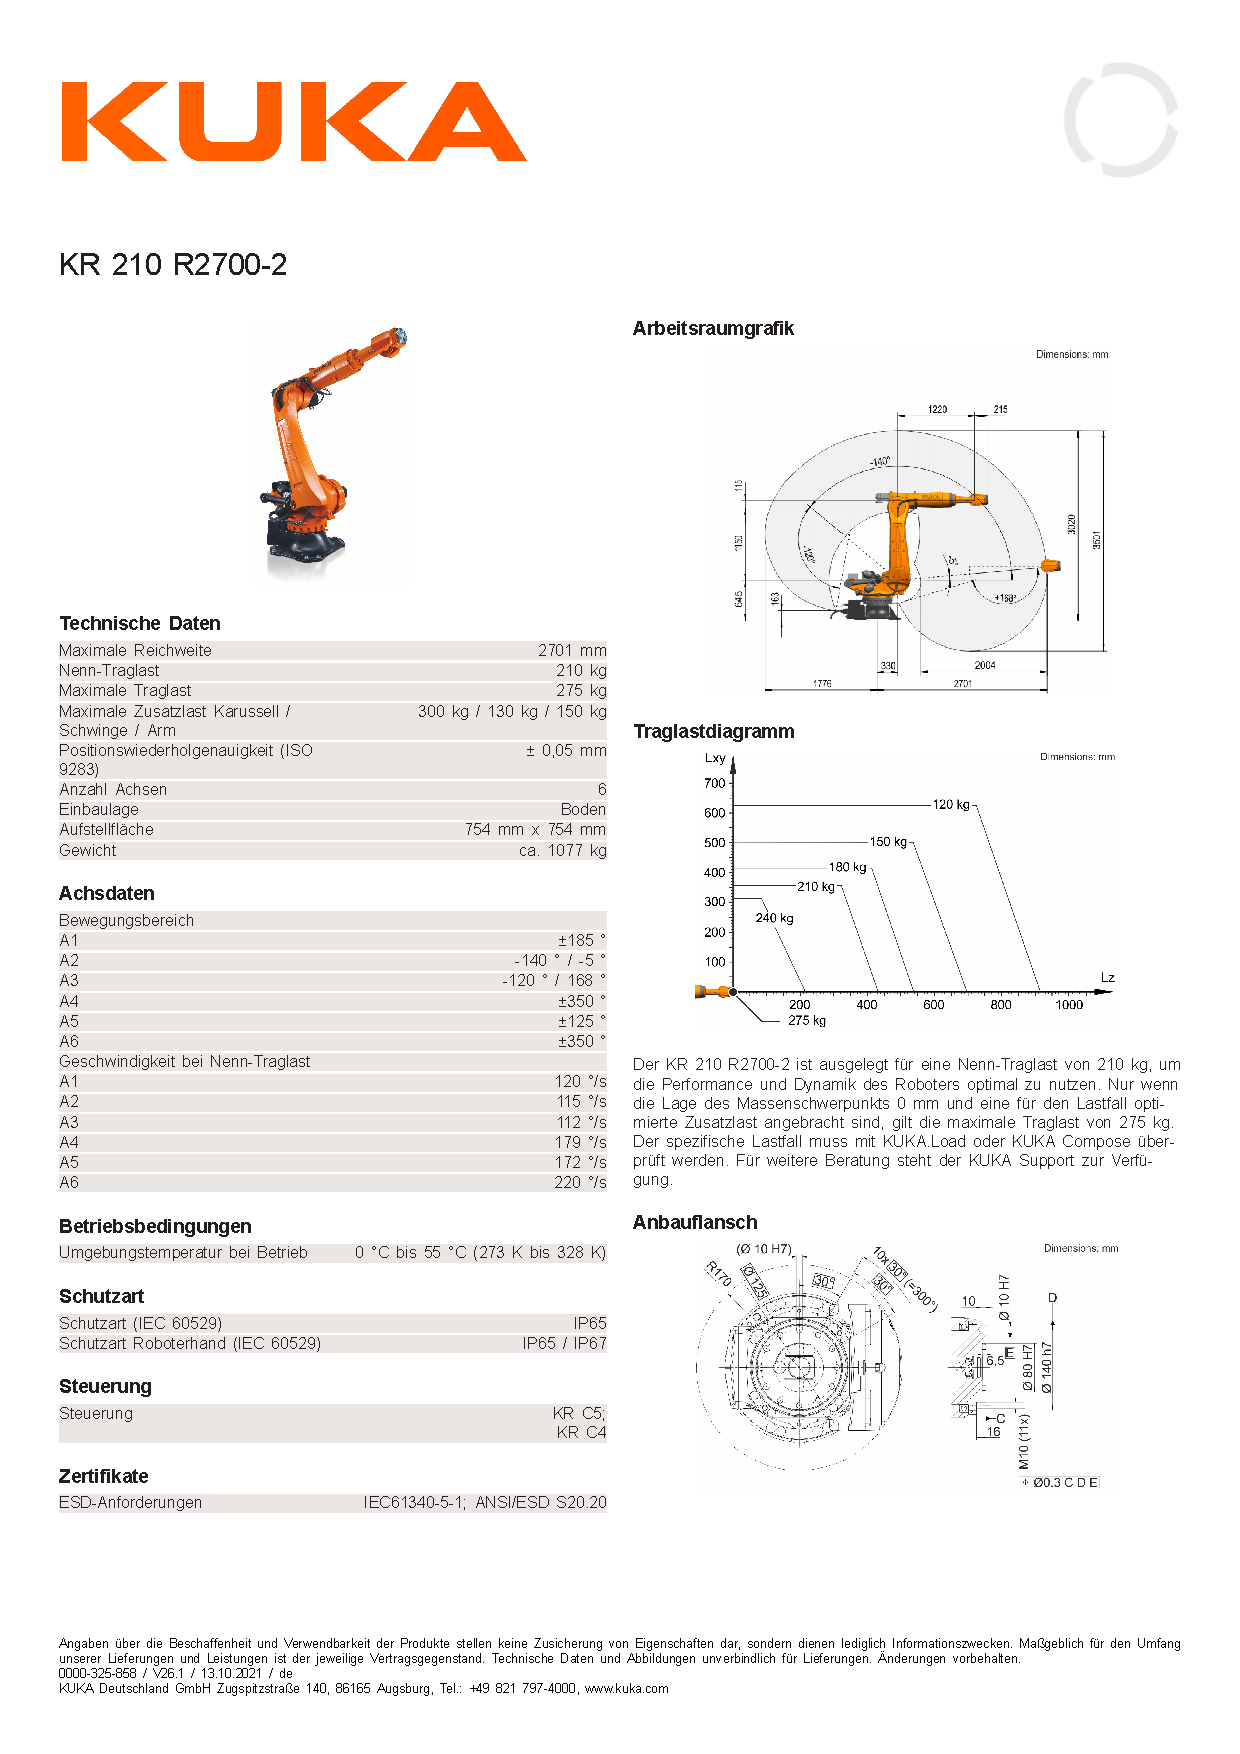
\includepdf[pages=1]{C:/Users/denni/Documents/Bachelorarbeit/BachelorThesis/literature/Anhang/DatenblattKR2102700-2.pdf}
%
\addchap{Anhang B}
\setcounter{chapter}{2}
\setcounter{section}{1}
\setcounter{table}{0}
\setcounter{figure}{0}
%
\section{DH-Transformation}
\label{add:dh}
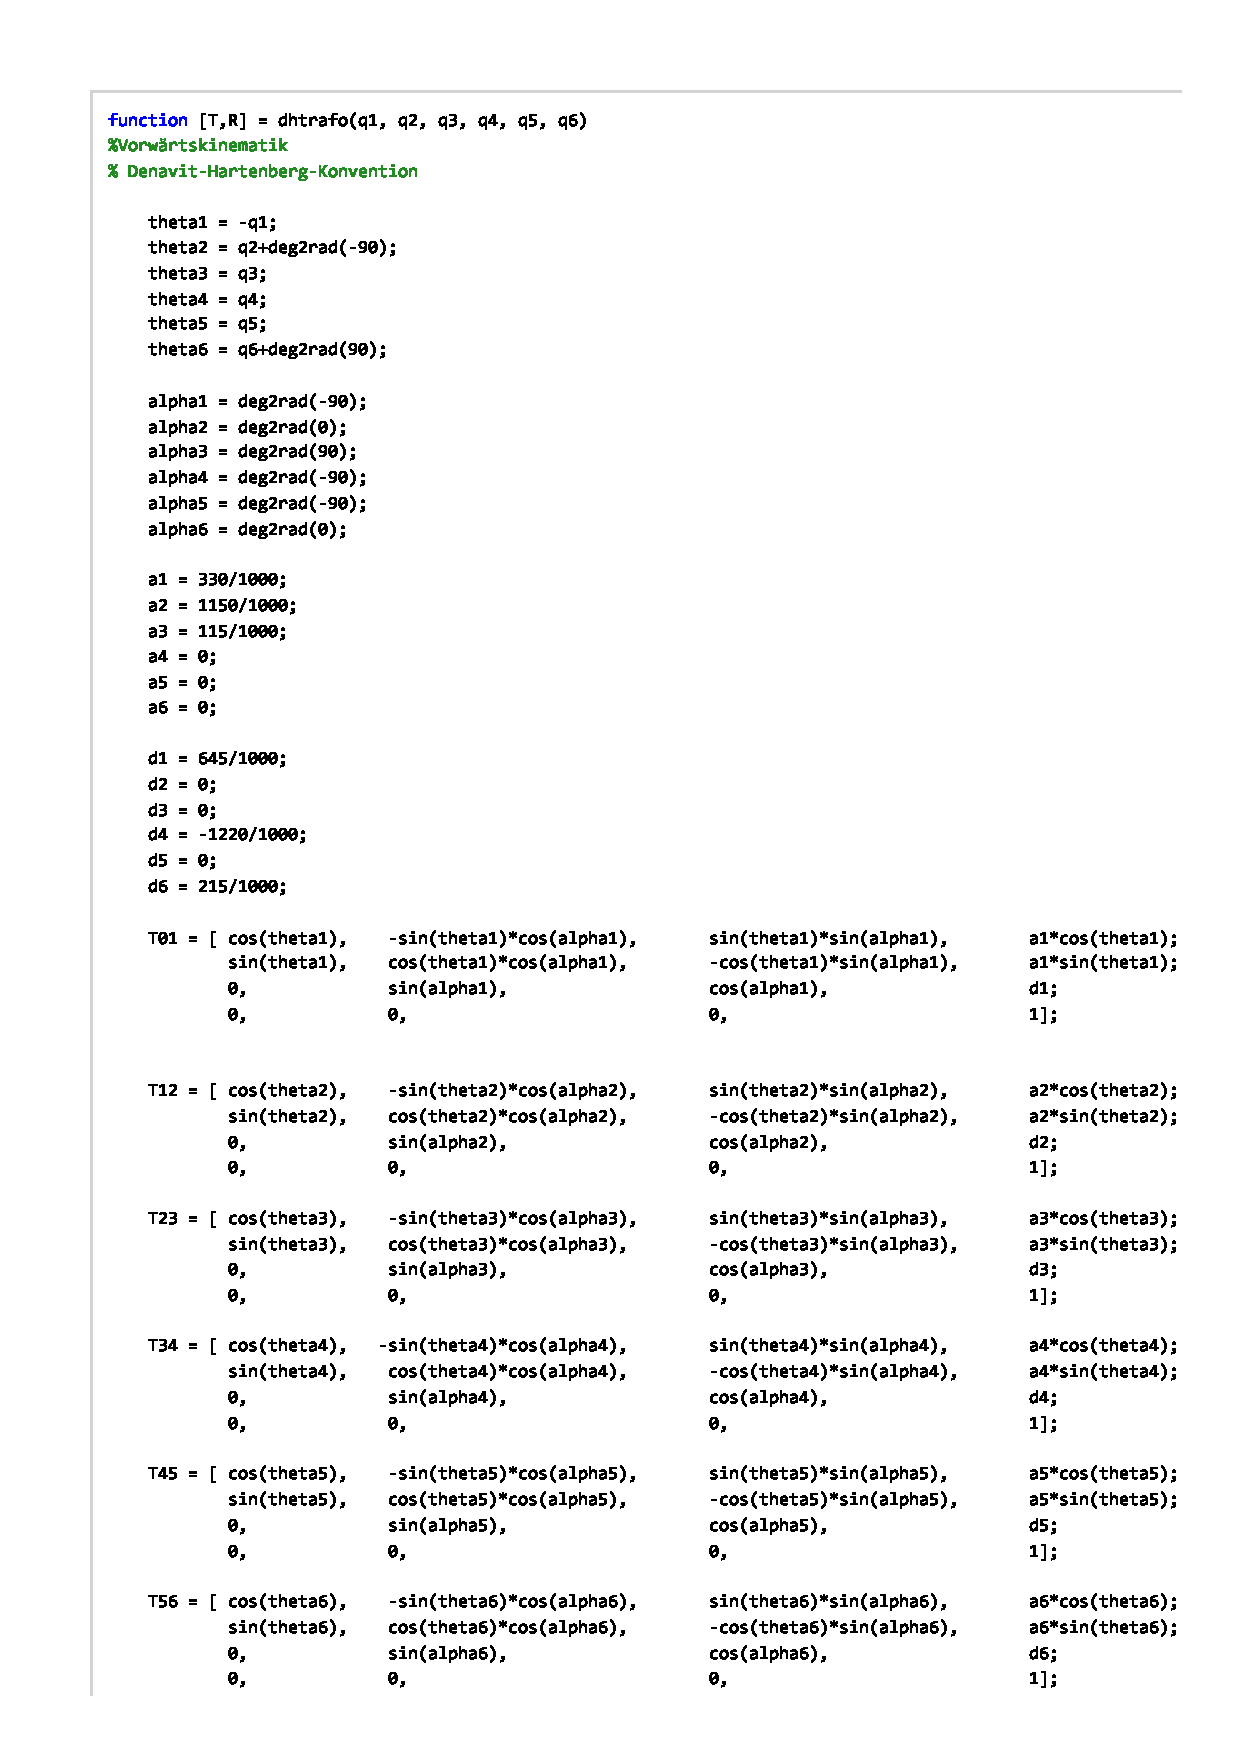
\includepdf[pages=1-2]{C:/Users/denni/Documents/Bachelorarbeit/BachelorThesis/literature/Anhang/dhtrafo_matlab.pdf}
%
\setcounter{chapter}{2}
\setcounter{section}{2}
\setcounter{table}{0}
\setcounter{figure}{0}
%
\label{add:systemparameter}
\section{Systemparameter}
Die Massen $m_i$ der Starrkörper $i$ sind dem CAD-Modell des Herstellers entnommen. Hierbei wird angenommen, dass der Werkstoff korrekt zugeordnet ist. 
%
\setlist{noitemsep}
\begin{itemize}
	\item $m_1$ = 535 kg
	\item $m_2$ = 696,3 kg
	\item $m_3$ = 361,6 kg
	\item $m_4$ = 39,676 kg
	\item $m_5$ = 53,619 kg
	\item $m_6$ = 4,528 kg
\end{itemize}
%
Die Trägheitstensoren, werden vom CAD-Modell, bezogen auf das KS$\left\{0\right\}$  vorgegeben. Gleichung \ref{eqn:similarity}  zeigt, wie diese einmalig über eine Ähnlichkeitstransformation auf das Körperfeste Koordinatensystem KS$\left\{i\right\}$ transformiert werden. Nachfolgend sind die Trägheitstensoren  bezogen auf das KS$\left\{0\right\}$ angegeben. 
%
\setlist{noitemsep}
\begin{itemize}
	\item $I_{1xx} = 17,298~\frac{\text{kg}}{\text{m}^2}$
	\item $I_{1xy} = -2,711~\frac{\text{kg}}{\text{m}^2}$
	\item $I_{1xz} = 1,672~\frac{\text{kg}}{\text{m}^2}$
	\item $I_{1yy} = 32,671~\frac{\text{kg}}{\text{m}^2}$
	\item $I_{1yz} = -0,493~\frac{\text{kg}}{\text{m}^2}$
	\item $I_{1zz} = 29,447~\frac{\text{kg}}{\text{m}^2}$
	\\
	\item $I_{2xx} = 138,135~\frac{\text{kg}}{\text{m}^2}$
	\item $I_{2xy} = -0,012~\frac{\text{kg}}{\text{m}^2}$
	\item $I_{2xz} = 0,387~\frac{\text{kg}}{\text{m}^2}$
	\item $I_{2yy} = 136,664~\frac{\text{kg}}{\text{m}^2}$
	\item $I_{2yz} = 9,231~\frac{\text{kg}}{\text{m}^2}$
	\item $I_{2zz} = 11,838~\frac{\text{kg}}{\text{m}^2}$
	\\
	\item $I_{3xx} = 3,031~\frac{\text{kg}}{\text{m}^2}$
	\item $I_{3xy} = -1,386~\frac{\text{kg}}{\text{m}^2}$
	\item $I_{3xz} = -0,045~\frac{\text{kg}}{\text{m}^2}$
	\item $I_{3yy} = 30,03~\frac{\text{kg}}{\text{m}^2}$
	\item $I_{3yz} = -0,21~\frac{\text{kg}}{\text{m}^2}$
	\item $I_{3zz} = 29,693~\frac{\text{kg}}{\text{m}^2}$
	\\
	\item $I_{4xx} = 0,099~\frac{\text{kg}}{\text{m}^2}$
	\item $I_{4xy} = -0,032~\frac{\text{kg}}{\text{m}^2}$
	\item $I_{4xz} = -0,001~\frac{\text{kg}}{\text{m}^2}$
	\item $I_{4yy} = 0,701~\frac{\text{kg}}{\text{m}^2}$
	\item $I_{4yz} = -9,367\cdot10^{-6}~\frac{\text{kg}}{\text{m}^2}$
	\item $I_{4zz} = 0,698~\frac{\text{kg}}{\text{m}^2}$
	\\
	\item $I_{5xx} = 0,481~\frac{\text{kg}}{\text{m}^2}$
	\item $I_{5xy} = 0,118~\frac{\text{kg}}{\text{m}^2}$
	\item $I_{5xz} = 0.00~\frac{\text{kg}}{\text{m}^2}$
	\item $I_{5yy} = 0,424~\frac{\text{kg}}{\text{m}^2}$
	\item $I_{5yz} = 0,00~\frac{\text{kg}}{\text{m}^2}$
	\item $I_{5zz} = 0,675~\frac{\text{kg}}{\text{m}^2}$
	\\
	\item $I_{6xx} = 0,011~\frac{\text{kg}}{\text{m}^2}$
	\item $I_{6xy} = 5,143\cdot10^{-7}~\frac{\text{kg}}{\text{m}^2}$
	\item $I_{6xz} = -2,003\cdot10^{-6}~\frac{\text{kg}}{\text{m}^2}$
	\item $I_{6yy} = 0,006~\frac{\text{kg}}{\text{m}^2}$
	\item $I_{6yz} = 1,220\cdot10^{07}~\frac{\text{kg}}{\text{m}^2}$
	\item $I_{6zz} = 0,006~\frac{\text{kg}}{\text{m}^2}$
\end{itemize}
%
Nachfolgend ist die Lage der Massenschwerpunkte $C_i^0$ im KS$\left\{0\right\}$ angegeben. 
% 
\begin{itemize}
	\item $r_{0,C_1}^0$ = $\left[-30,103,~441,~452,213\right]$ mm
	\item $r_{0,C_2}^0$ = $\left[330,979,~-222,585,~1094,239\right]$ mm
	\item $r_{0,C_3}^0$ = $\left[705,894,~-8,126,~1908,436\right]$ mm
	\item $r_{0,C_4}^0$ = $\left[1383,185,~4,492,~1909,983\right]$ mm
	\item $r_{0,C_5}^0$ = $\left[1601,767,~33,833,~1909,955\right]$ mm
	\item $r_{0,C_6}^0$ = $\left[1743,222,~-0,007,~1910 051\right]$ mm
\end{itemize}
%
Die Getriebeübersetzung ist der Datei Machine Data (MADA) der Robotersteuerung entnommen.
%
\begin{itemize}
	\item $i_1 = \frac{-7}{1798}$
	\item $i_2 = \frac{17}{4576}$
	\item $i_3 = \frac{3}{754}$
	\item $i_4 = \frac{-55}{10387}$
	\item $i_5 = \frac{-483}{91834}$
	\item $i_6 = \frac{49400}{6485103}$
\end{itemize}
 %
Nachfolgend ist die Umsetzung der Parameter Transformation via MATLAB\textsuperscript{\textregistered} gezeigt. 
%
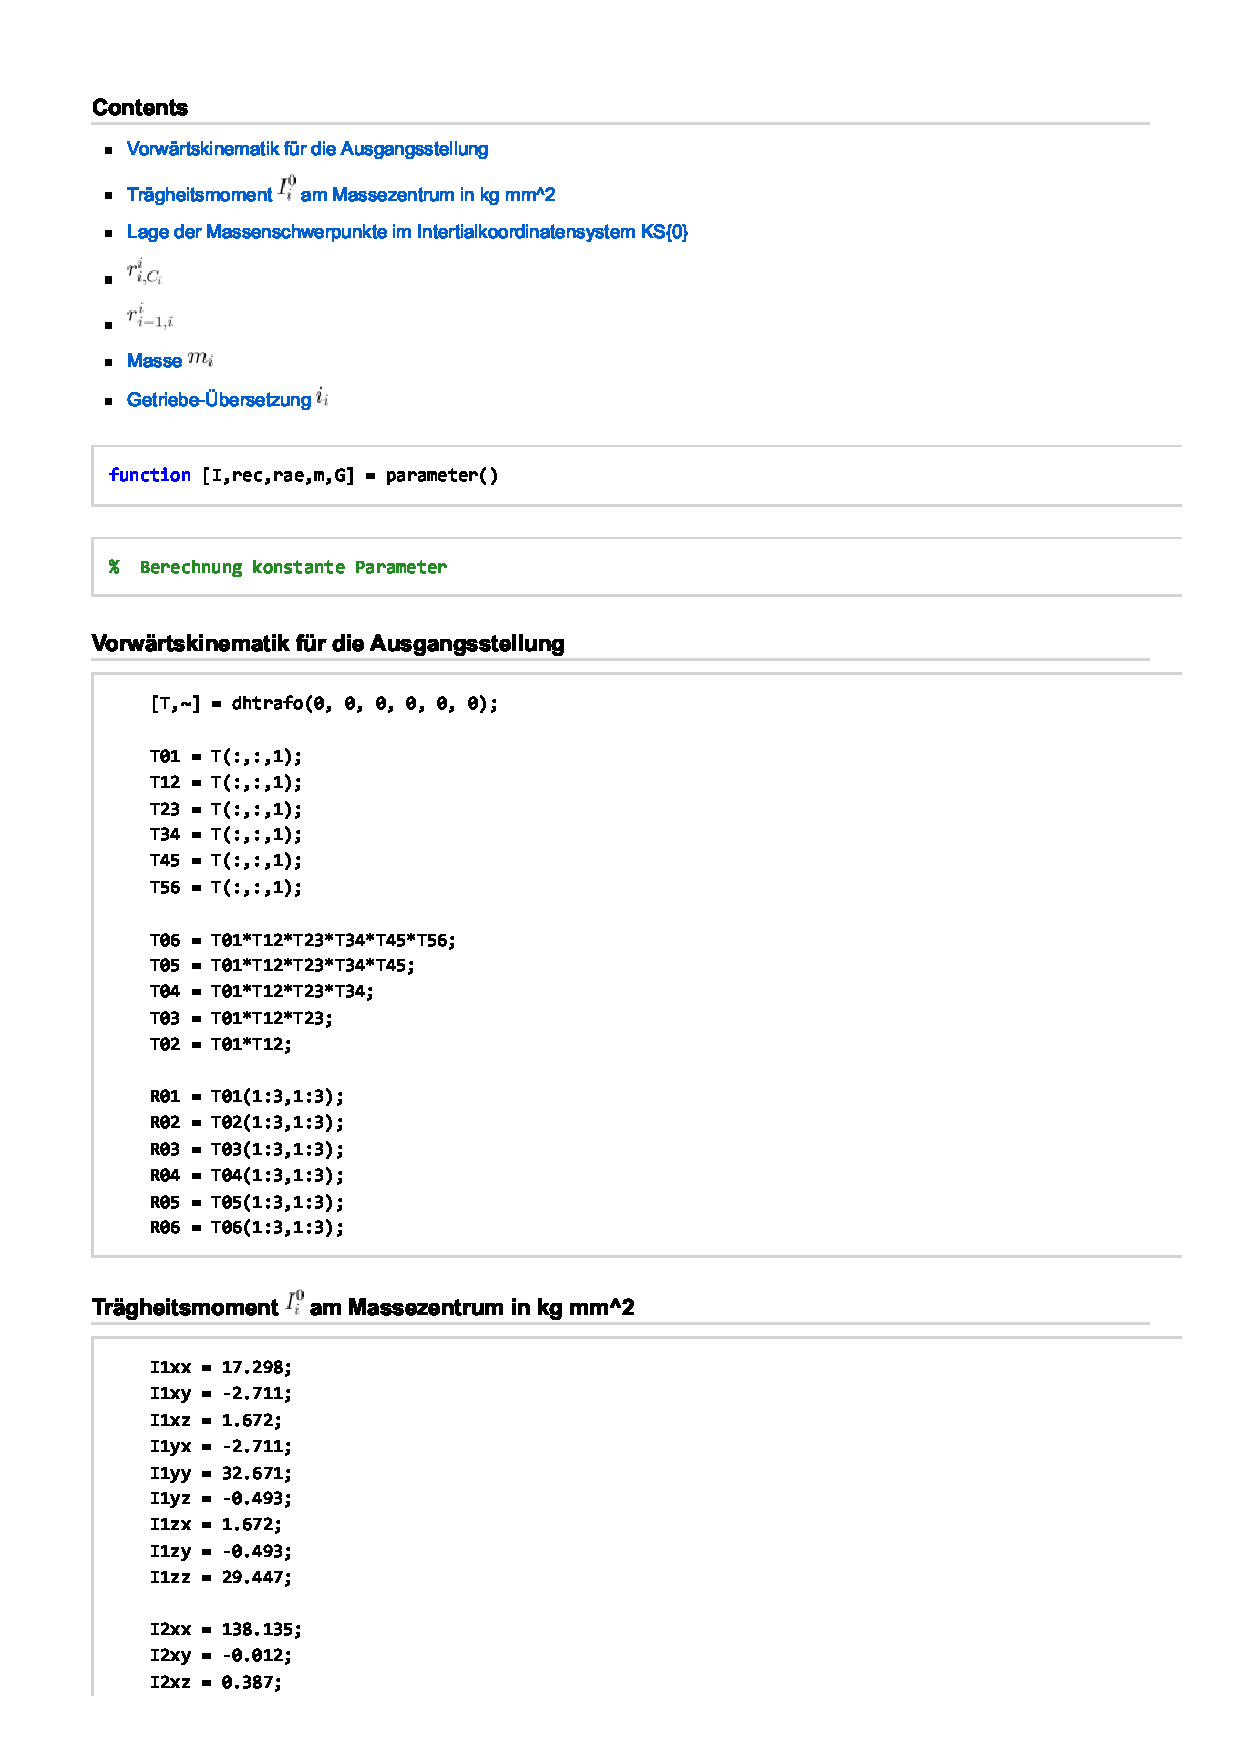
\includepdf[pages=1-4]{C:/Users/denni/Documents/Bachelorarbeit/BachelorThesis/literature/Anhang/parameter_matlab.pdf}
%
\setcounter{chapter}{2}
\setcounter{section}{3}
\setcounter{table}{0}
\setcounter{figure}{0}
%
\section{RNEA}
\label{add:rnea}
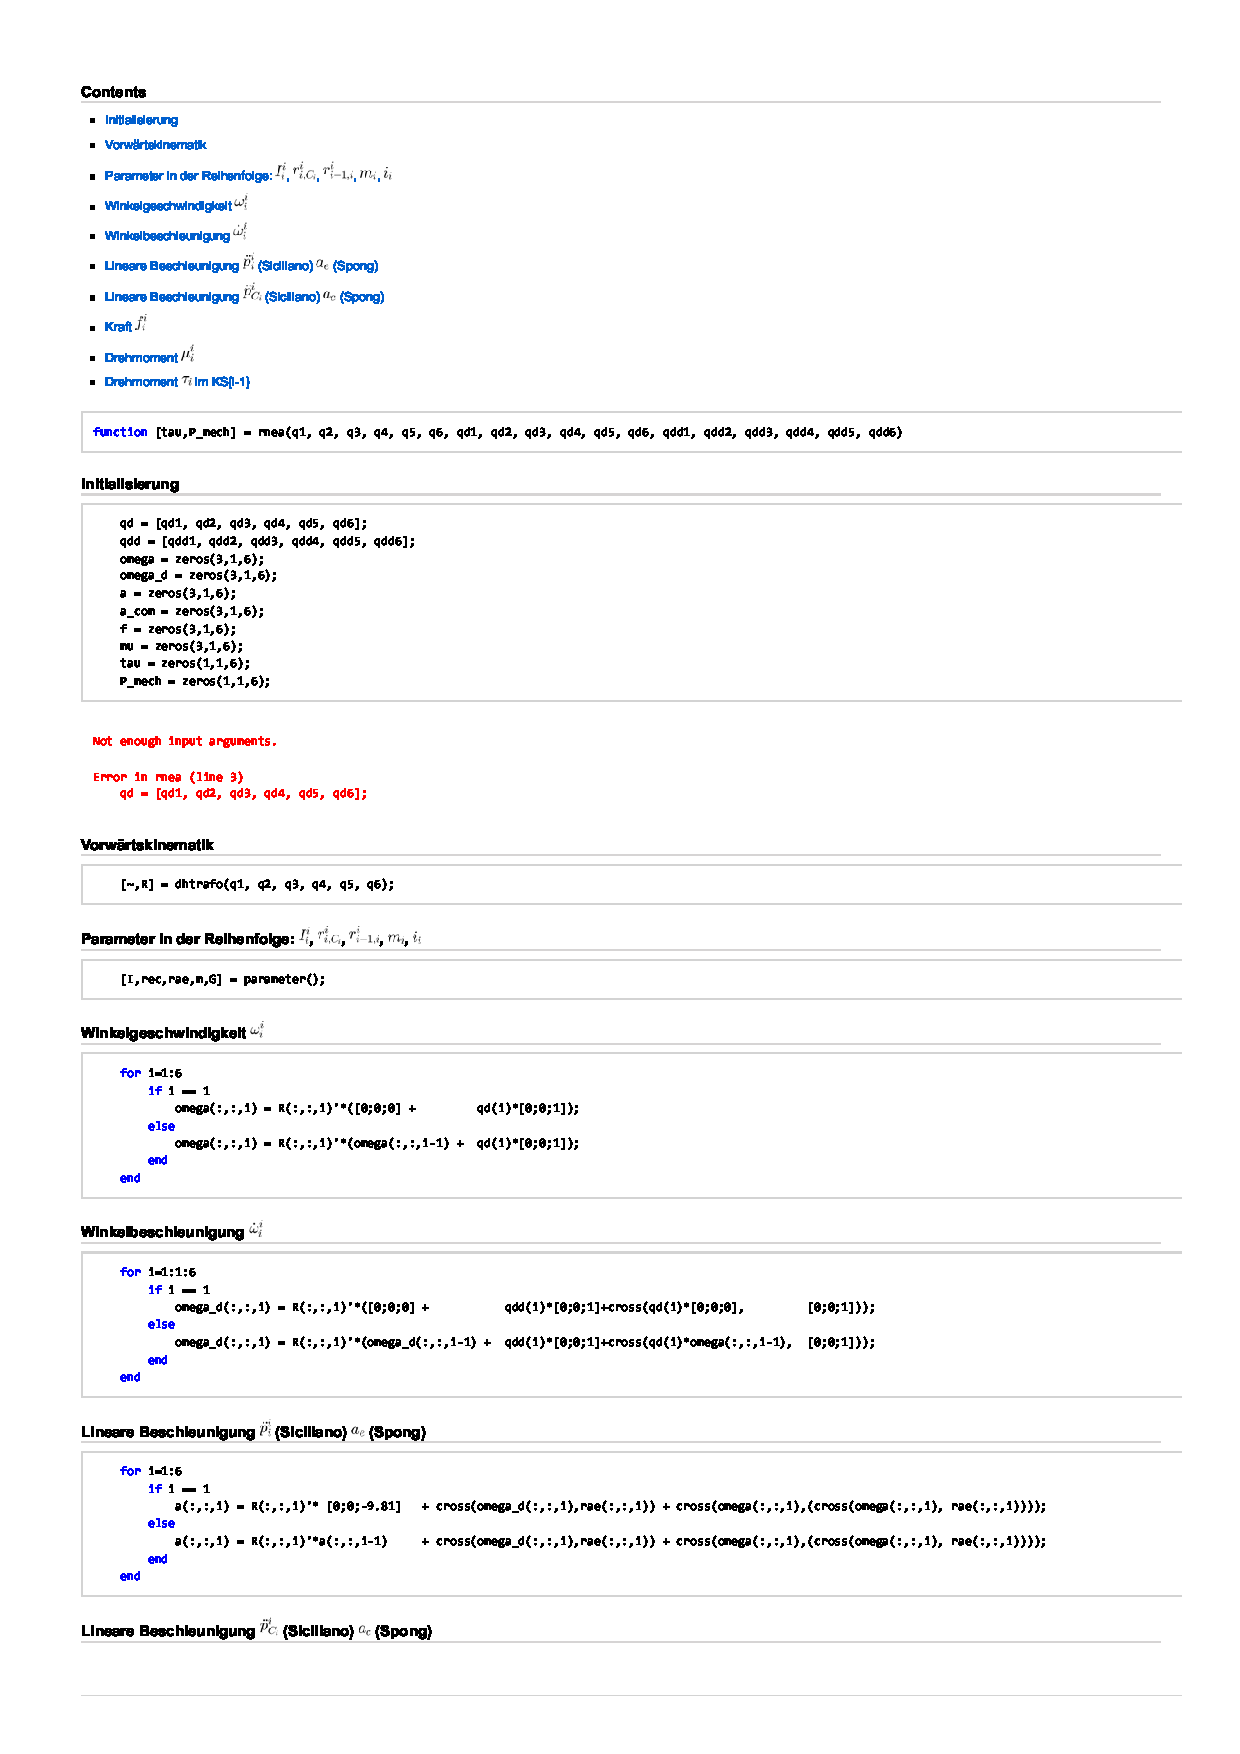
\includepdf[pages=1-2]{C:/Users/denni/Documents/Bachelorarbeit/BachelorThesis/literature/Anhang/rnea_matlab.pdf}
%
\setcounter{chapter}{2}
\setcounter{section}{4}
\setcounter{table}{0}
\setcounter{figure}{0}
%
\section{Bahnplanung}
\label{add:traj}
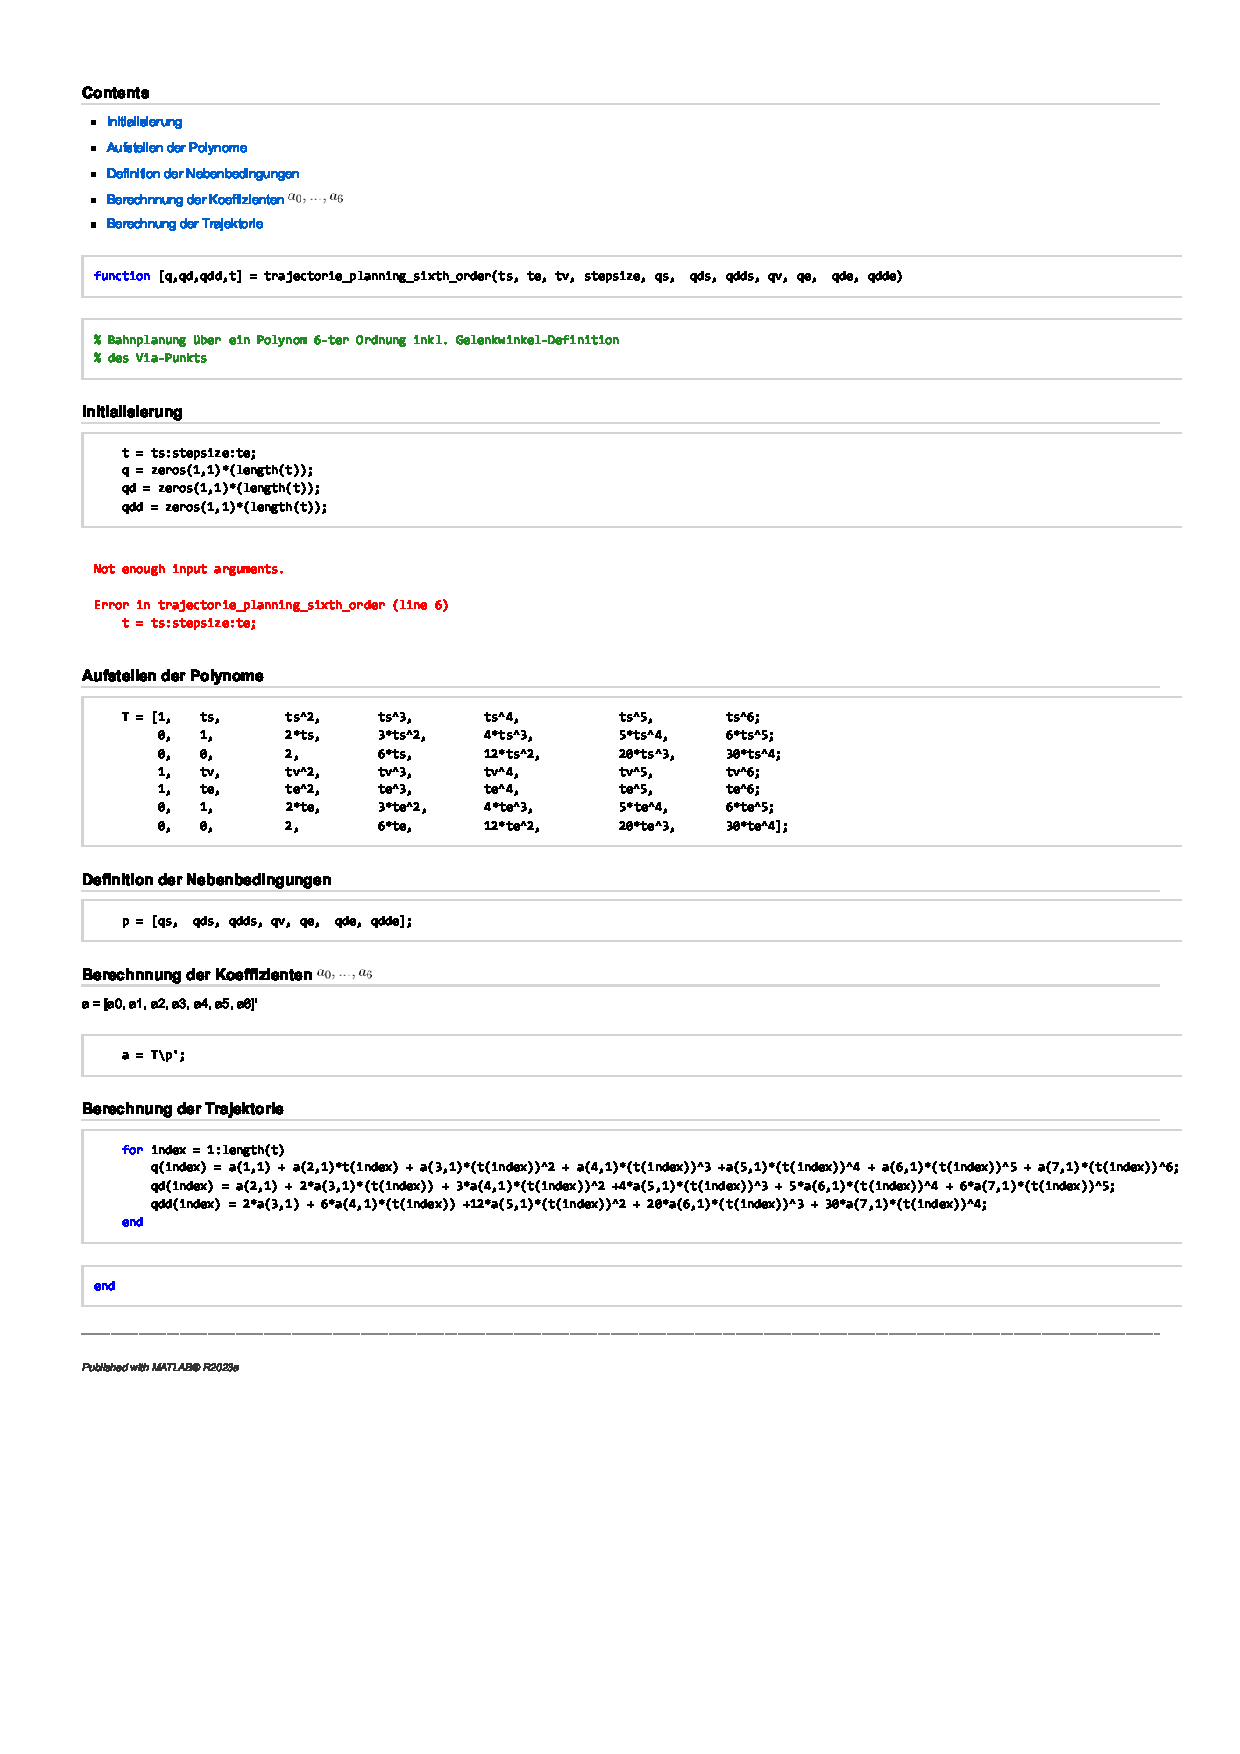
\includepdf[pages=1]{C:/Users/denni/Documents/Bachelorarbeit/BachelorThesis/literature/Anhang/trajectorie_planning_sixth_order_matlab.pdf}
%
\setcounter{chapter}{2}
\setcounter{section}{5}
\setcounter{table}{0}
\setcounter{figure}{0}
%
\section{Testsimulation Bahnplanung}
\label{add:sim}
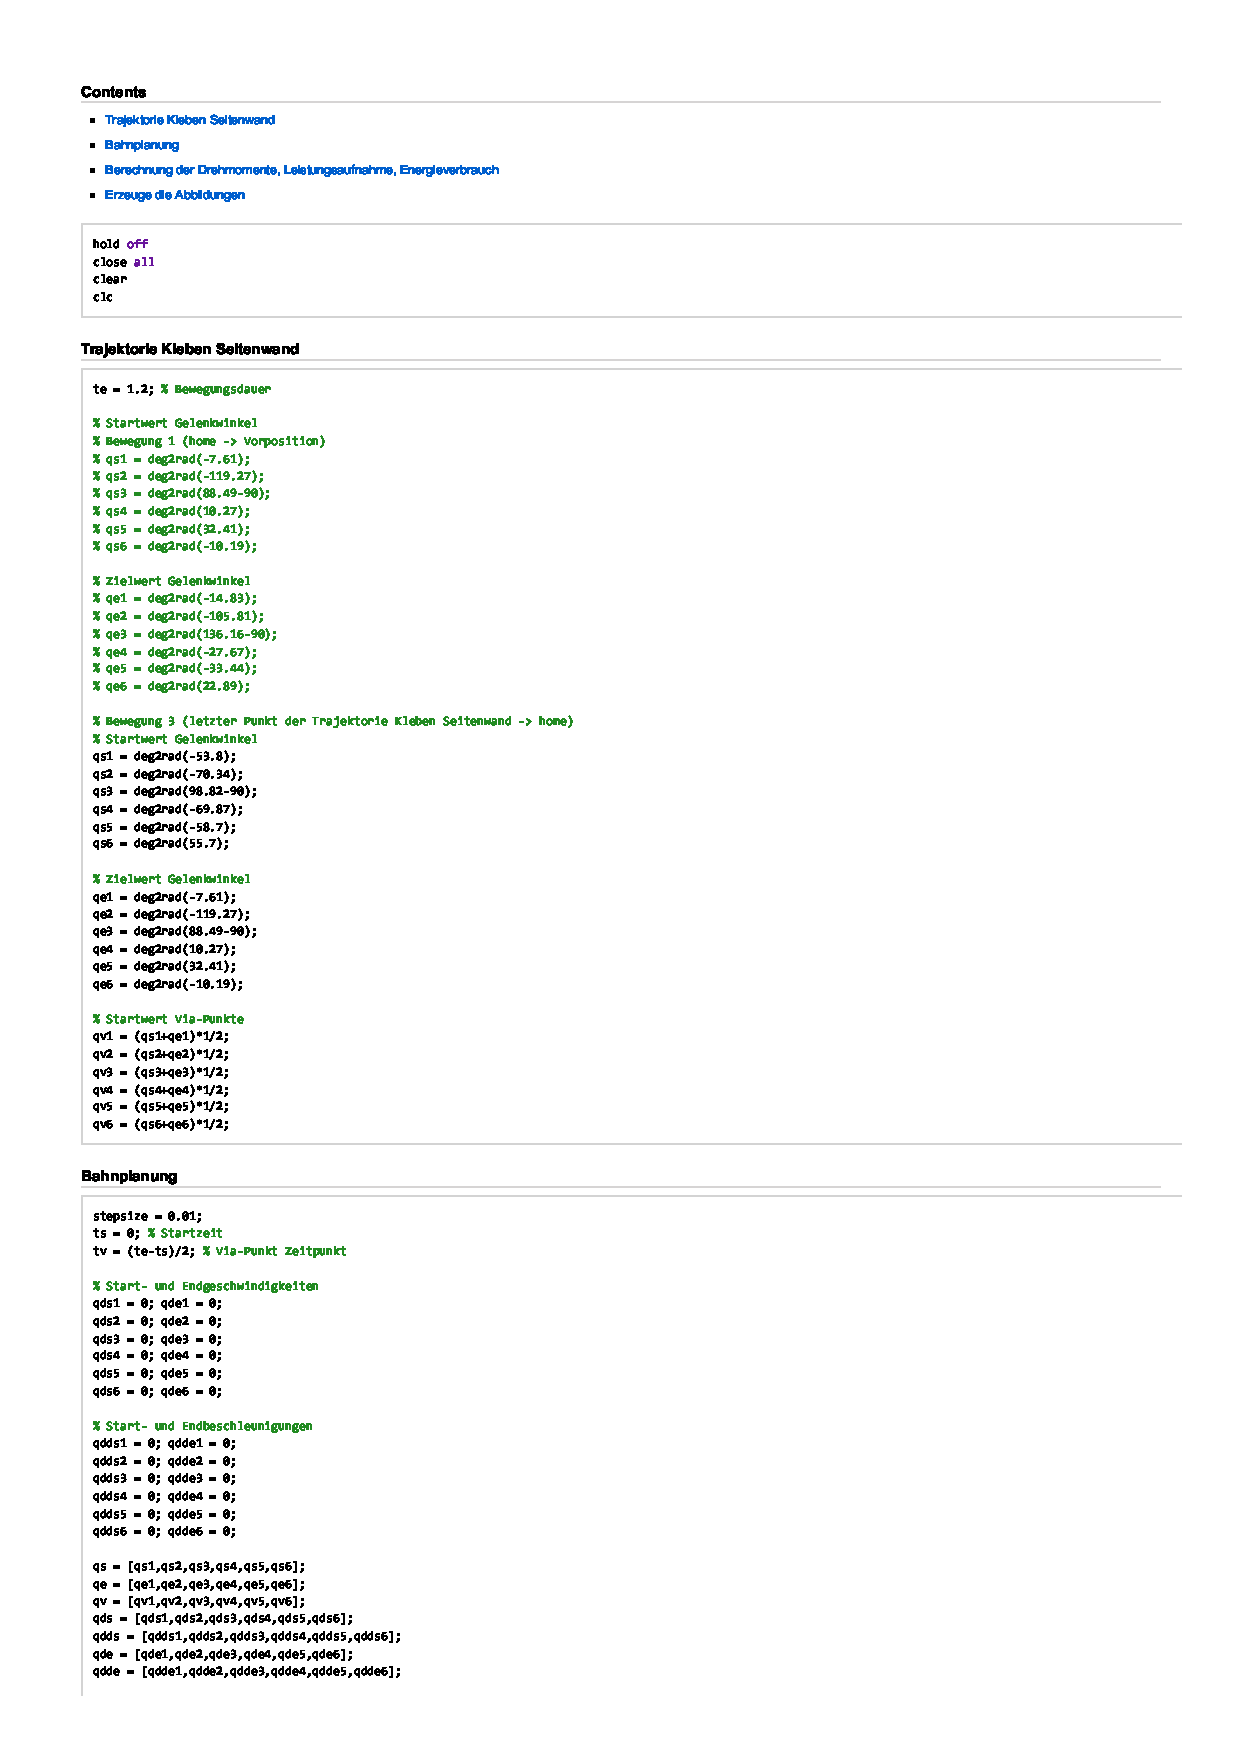
\includepdf[pages=1-2]{C:/Users/denni/Documents/Bachelorarbeit/BachelorThesis/literature/Anhang/simulation_matlab.pdf}
%
\setcounter{chapter}{2}
\setcounter{section}{5}
\setcounter{table}{0}
\setcounter{figure}{0}
%
\section{Grafische Ausgabe}
\label{add:plot}
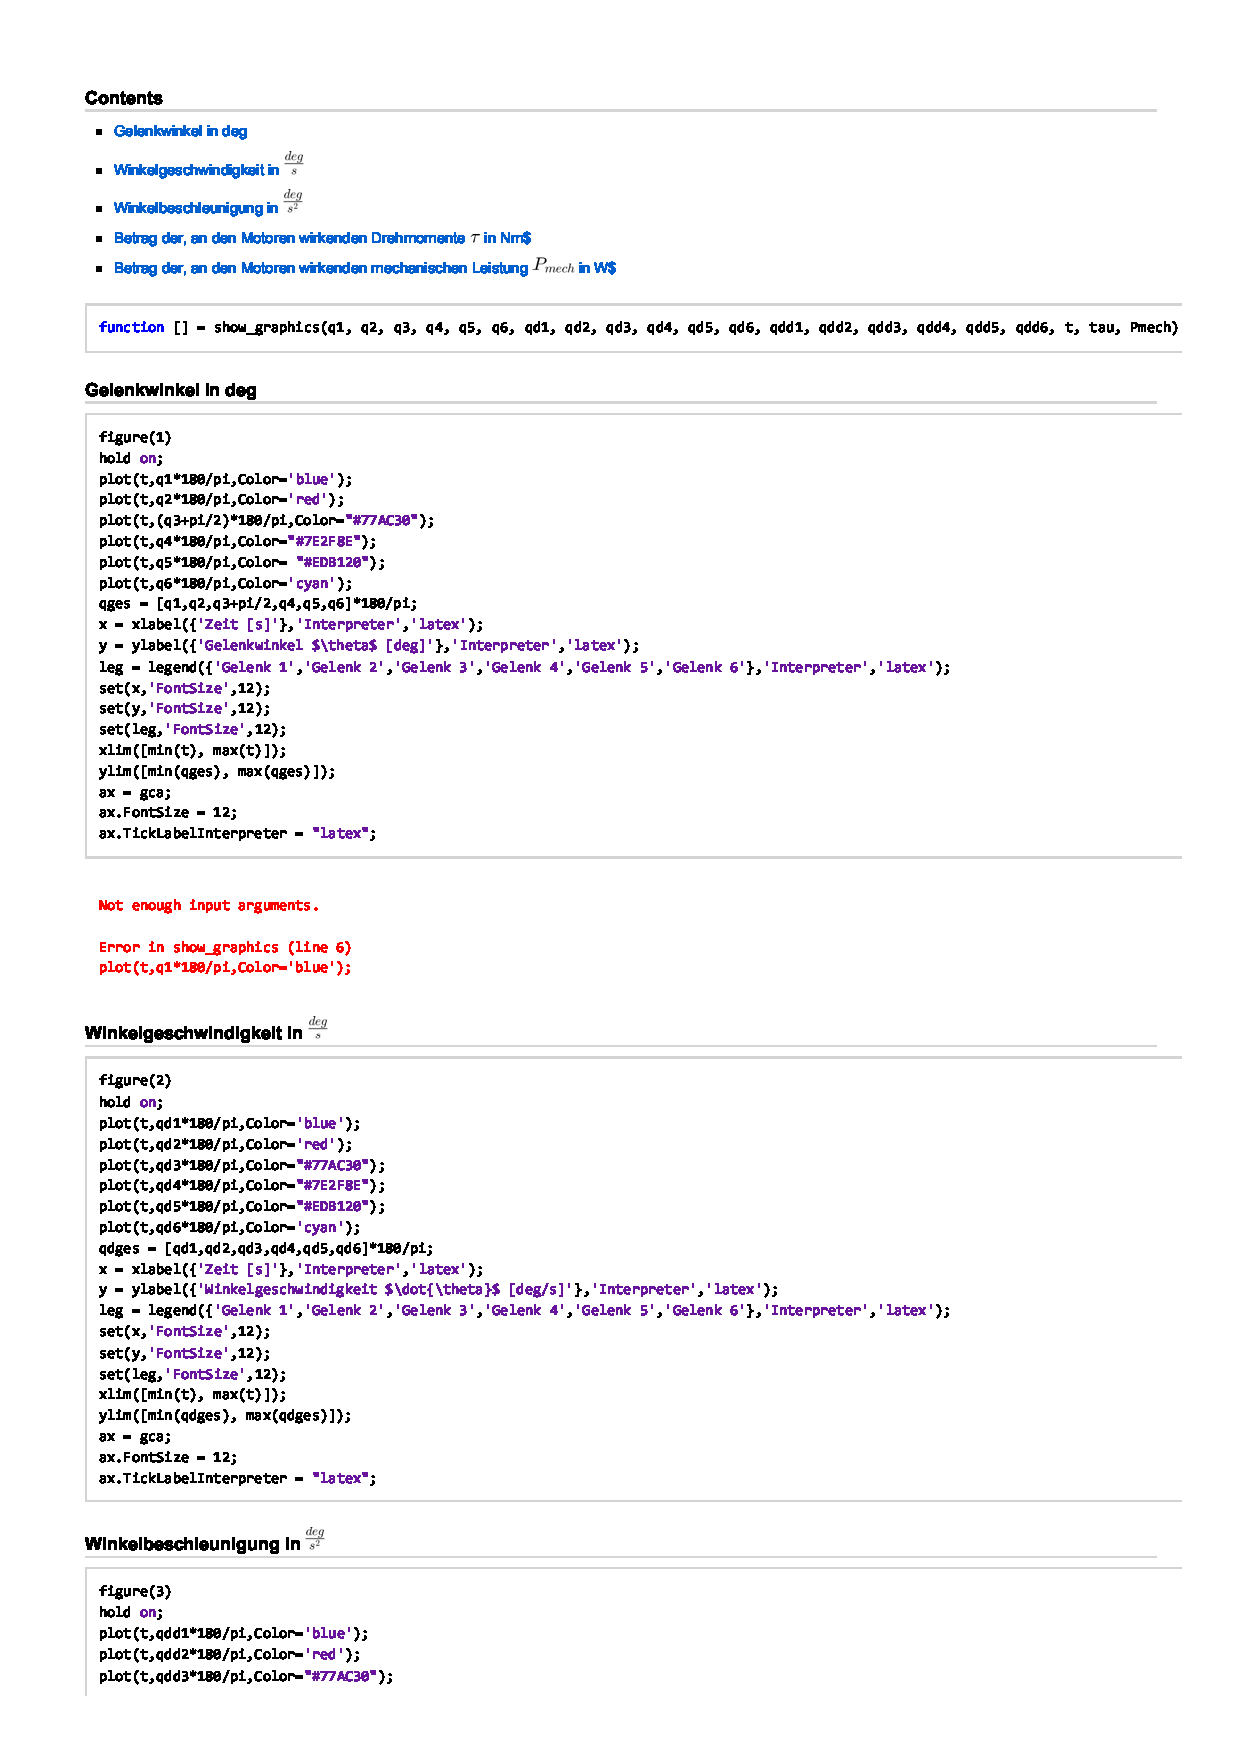
\includepdf[pages=1-2]{C:/Users/denni/Documents/Bachelorarbeit/BachelorThesis/literature/Anhang/show_graphics_matlab.pdf}
